\label{user}
%%%%%%%%%%%%%%%%%%%%%%%%%%%%%%%%%%%%%%%%%%%%%%%%%%%%%%%%%%%%%%%%%%
%%%%%%%%%%%%%%%%%%%%%%%%%%%%%%%%%%%%%%%%%%%%%%%%%%%%%%%%%%%%%%%%%%

\subsection{Introduction}
Pour rappel, notre \acrshort{os} est exécuté sur architecture Intel 32-bits (\acrshort{IA-32})
en mode protégé. Dans cette architecture, quatre niveaux de privilèges existent.
Nous avons déjà fait référence aux niveaux de privilèges (ou \textit{ring})
dans ce document quand les différentes tables de descripteurs ont été décrites
(chapitres \ref{gdt_ldt} sur la \acrshort{gdt} et la \acrshort{ldt} et \ref{idt}
sur l'\acrshort{idt}). Les niveaux de privilèges vont de 0 à 3. Le \textit{ring}
0 (\textit{kernel}) a le plus de privilèges et peut accéder à tout le jeu d'instructions
du processeur alors que le \textit{ring} 3 (\textit{user}) en a le moins et a accès
à un jeu d'instructions restreint \cite{ref42}.

\begin{figure}[!h]
  \centering
  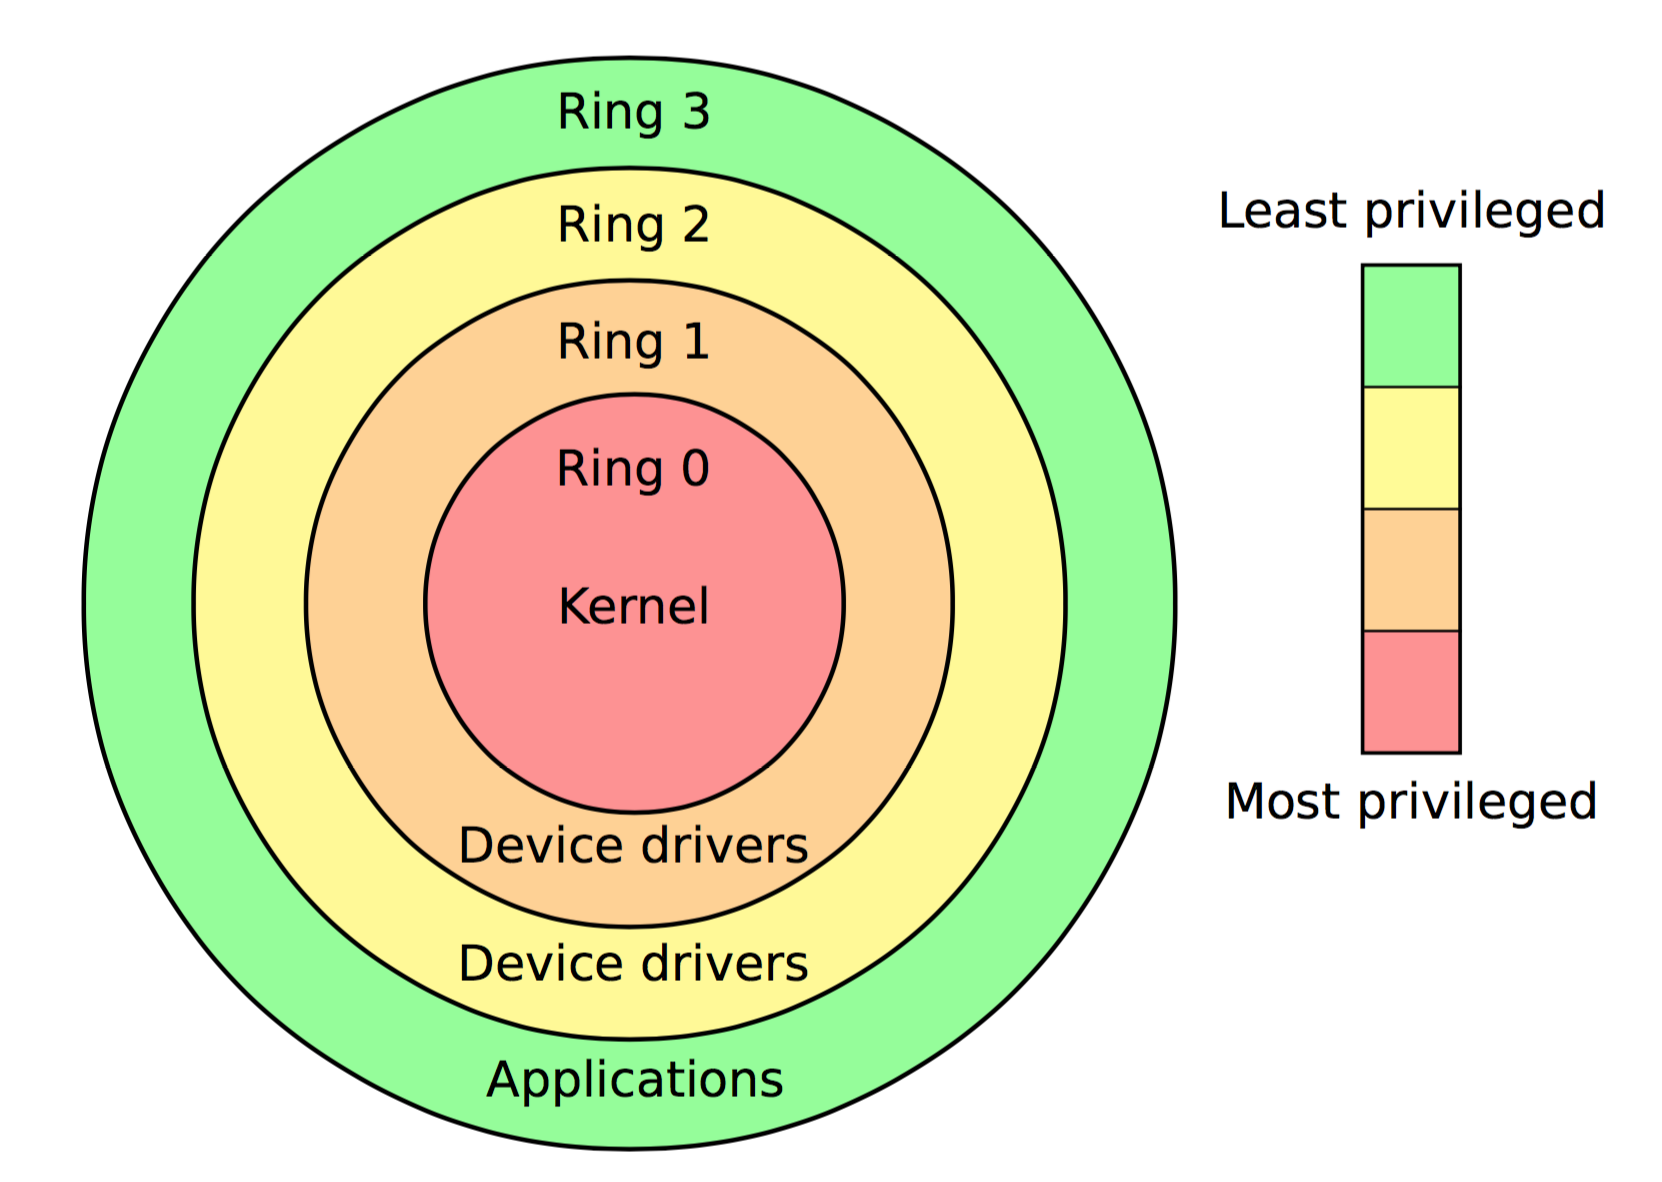
\includegraphics[scale=.4]{images/rings.png}
  \caption{Niveaux de privilèges sur architecture \acrshort{IA-32}}
  \label{rings}
\end{figure}

Le \textit{ring} 0 est aussi appelé mode privilégié. Ce mode peut accéder aux régions
privilégiées de la mémoire (définies lors de l'initialisation de la \acrshort{gdt}
ou de la pagination). Seulement ce mode peut contrôler le \acrshort{mmu}, accéder
aux périphériques, définir les vecteurs d'interruptions ou encore arrêter le
processeur. L'\acrshort{os} démarre en mode privilégié car le \textit{kernek} doit
pouvoir accéder au matériel sans aucune restriction. Si ce n'était pas le cas toutes
les configurations de la mémoire et des périphériques décrites dans ce document
auraient été impossibles. En revanche, Les applications utilisateur s'exécutent
en mode utilisateur (\textit{ring} 3). Si une application utilisateur démarrait
avec le niveau de privilèges maximal, elle pourrait écrire dans les régions mémoires
du \textit{kernel}, modifier la configuration de la mémoire (\acrshort{gdt} ou 
répertoire de pages) ou encore changer l'\acrshort{idt}. Il est donc impératif
d'exécuter les applications en \textit{ring} 3. Grâce à ce mécanisme de protection,
le \textit{kernel} peut être complètement isolé des applications. Le rôle du \textit{kernel}
est dans un premier temps d'attribuer et de gérer l'espace mémoire de chaque application.
Il doit ensuite programmer correctement le processeur pour isoler les tâches exécutées
et assurer le bon fonctionnement du système.

%%%%%%%%%%%%%%%%%%%%%%%%%%%%%%%%%%%%%%%%%%%%%%%%%%%%%%%%%%%%%%%%%%
%%%%%%%%%%%%%%%%%%%%%%%%%%%%%%%%%%%%%%%%%%%%%%%%%%%%%%%%%%%%%%%%%%

\subsection{Exécution d'une tâche}
\subsubsection{Structure d'une tâche}
L'architecture \acrshort{IA-32} implémente la gestion des tâches au niveau matériel.
Une tâche doit être constituée d'un espace d'exécution et d'une structure \acrshort{tss}.
L'espace d'exécution est constitué d'un segment de code, d'un segment de données
et d'un segment de pile. La manière dont ces segments sont définis dépend de la
méthode de gestion mémoire utilisée. Si la pagination n'est pas utilisée, ces segment
seront définis par une \acrshort{ldt}. Avant d'implémenter la pagination, cette
méthode était utilisée par notre \textit{kernel} pour gérer l'espace d'adressage
d'une tâche. Avec la pagination, deux segments en \textit{ring} 3 sur tout l'espace
d'adressage suffisent (un segment de code et un segment de données). Ces segments
sont identiques à ceux déjà construits pour le \textit{kernel} et décrits dans
la partie \ref{gdt_ldt} à la différence qu'ils n'ont pas le même niveau de privilèges.
Ainsi, une tâche a théoriquement un espace d'exécution de 4Go (taille de la \acrshort{ram}).
En réalité, l'espace d'exécution de la tâche est défini par un répertoire de pages
(différent de celui du \textit{kernel}) où seront allouées autant de pages qu'il faut
pour contenir l'application utilisateur. C'est la structure \acrshort{tss} qui spécifie
les segments définissant l'espace d'exécution. Si la pagination n'est pas utilisée,
c'est dans cette structure que le sélecteur vers la \acrshort{ldt} doit être spécifié.
Dans le cas contraire, le \acrshort{tss} contient aussi un champs \mintinline{rust}{cr3}
pour définir le répertoire de pages de la tâche (voir figure \ref{task_exec_space})
\cite{ref66}.

\begin{figure}[!h]
  \centering
  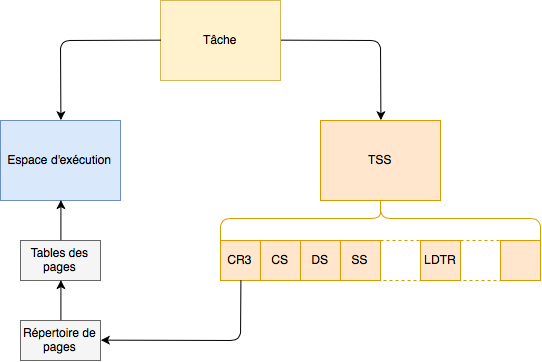
\includegraphics[scale=.7]{images/task_exec_space.png}
  \caption{Structure d'une tâche avec la pagination}
  \label{task_exec_space}
\end{figure}

La structure \acrshort{tss} permet aussi de sauvegarder le contexte de la tâche
dans le cas où une tâche en appelle une autre. Chaque \acrshort{tss} a un descripteur
dans la \acrshort{gdt}. Il y a donc autant de descripteurs de \acrshort{tss} dans
la \acrshort{gdt} que de tâches. Une tâche est alors identifiée par le sélecteur
de segment référençant son \acrshort{tss} dans la \acrshort{gdt} \cite{ref42}. Etant
donné que la pagination est utilisée dans la version finale de notre \acrshort{os},
nous allons nous concentrer sur la gestion des tâches utilisant un répertoire de
pages.

%%%%%%%%%%%%%%%%%%%%%%%%%%%%%%%%%%%%%%%%%%%%%%%%%%%%%%%%%%%%%%%%%%

\subsubsection{Commutation de tâche}
Nous avons vu dans la partie précédente qu'une tâche est divisée en deux parties,
son espace d'exécution et sa structure \acrshort{tss}. Le processeur fourni un
mécanisme permettant de sauvegarder le contexte de la tâche courante et de commuter
vers une nouvelle tâche. La sauvegarde du contexte se fait en utilisant le \acrshort{tss}
lié à la tâche à exécuter et plus particulièrement le sélecteur de ce \acrshort{tss}
dans la \acrshort{gdt}. Ce dernier doit être donné commer argument à l'instruction
\mintinline{text}{ltr}. Cette instruction permet de charger le sélecteur de \acrshort{tss}
dans un registre spécial, le \textit{task register}. Ce registre indique au processeur
quelle est la tâche courante. Lorsqu'une commutation de tâche a lieu, l'état
courant du processeur est automatiquement sauvegardé dans le \acrshort{tss} pointé
par le \textit{task register}. Il est donc nécessaire de créer un \acrshort{tss}
initial avant d'exécuter la première tâche car l'état du processeur doit être
sauvegardé \cite{ref42}. Ci-dessous, la structure \acrshort{tss} en rust.

\begin{code}
\begin{minted}[fontsize=\footnotesize,tabsize=4,frame=single,linenos]{rust}
pub struct Tss {
    previous_task_link : u16, reserved0    : u16,
    esp0               : u32,
    ss0                : u16, reserved1    : u16,
    esp1               : u32,
    ss1                : u16, reserved2    : u16,
    esp2               : u32,
    ss2                : u16, reserved3    : u16,
    cr3                : u32,
    eip                : u32, eflags       : u32, eax: u32, ecx: u32, edx: u32,
    ebx                : u32, esp          : u32, ebp: u32, esi: u32, edi: u32,
    es                 : u16, reserved4    : u16,
    cs                 : u16, reserved5    : u16,
    ss                 : u16, reserved6    : u16,
    ds                 : u16, reserved7    : u16,
    fs                 : u16, reserved8    : u16,
    gs                 : u16, reserved9    : u16,
    ldt_selector       : u16, reserved10   : u16,
    reserved11         : u16,
    iomap_base_addr    : u16
}
\end{minted}
\caption{Champs de la structure \acrshort{tss}}
\label{lst:tasks:tss}
\end{code} \bigbreak

Dans le \acrshort{tss} initial, seuls les champs \mintinline{rust}{esp0},
\mintinline{rust}{ss0} et \mintinline{rust}{cr3} sont utilisés. Les champs
\mintinline{rust}{esp0} et \mintinline{rust}{ss0} sont utilisés pour stocker
la pile pour le niveau de privilèges 0 et \mintinline{rust}{cr3} doit pointer
sur le répertoire de pages du \textit{kernel}. Ce \acrshort{tss} est ensuite chargé
dans le \textit{task register} avec l'instruction \mintinline{text}{ltr}. Le
\textit{kernel} peut maintenant exécuter une tâche utilisateur. L'architecture
\acrshort{IA-32} offre de nombreux mécanismes pour commuter vers une nouvelle
tâche. La méthode utilisée est un appel explicite à la tâche avec l'instruction
\mintinline{text}{call far}. Cette instruction prend comme argument le sélecteur
du \acrshort{tss} de la tâche à exécuter (comme l'instruction \mintinline{text}{ltr}).
L'initialisation du \acrshort{tss} d'une tâche est légèrement plus complexe que
celle du \acrshort{tss} initial. Les sélecteurs de segment doivent pointer sur les
bons segments dans la \acrshort{gdt}. De plus, le pointeur d'exécution doit
pointer là où commence le code du programme utilisateur et les champs \mintinline{rust}{ss},
\mintinline{rust}{esp} et \mintinline{rust}{ebp} sont utilisés pour stocker la pile
pour le niveau de privilèges 3. L'adresse du début du programme utilisateur dépend
de la manière dont le répertoire de pages de la tâche a été initialisé. Dans notre
cas, le programme utilisateur commence toujours à l'adresse 0x0. Un programme
utilisateur contenu par exemple dans le disque dur peut ainsi être exécuté en
\textit{ring} 3.

%%%%%%%%%%%%%%%%%%%%%%%%%%%%%%%%%%%%%%%%%%%%%%%%%%%%%%%%%%%%%%%%%%
%%%%%%%%%%%%%%%%%%%%%%%%%%%%%%%%%%%%%%%%%%%%%%%%%%%%%%%%%%%%%%%%%%

\subsection{Appels systèmes}
Les appels systèmes sont des fonctions exposées aux applications utilisateur par
le \textit{kernel}. Lors d'un appel système, un changement de privilèges a lieu
car du code du \textit{kernel} est appelé. Il est important d'avoir des appels
systèmes dans un \textit{kernel} appelant des applications utilisateurs car
un programme utilisateur ne pourrait que modifier des variables et appeler des
fonctions s'il ne pouvait pas appeler du code au niveau du \textit{kernel}. Prenons
par exemple un simple affichage texte. Le programme utilisateur étant isolé du reste
de la mémoire, il ne peut pas accéder à la \acrshort{vram} et par conséquent ne
peut rien afficher à l'écran. Les appels systèmes se présentent donc comme une
\acrshort{api} de l'\acrshort{os}. Le mécanisme permettant à du code exécuté en
mode utilisateur d'appeler du code en mode \textit{kernel}
est réalisé grâce à une interruption logicielle choisie et configurée par le \textit{kernel}.
Cette interruption est configurée afin d'être exécutable en \textit{ring} 3.
Dans le cas de notre \textit{kernel}, l'interruption utilisée est la première libre
après les interruptions matérielles. C'est l'interruption 48. Sa configuration se
fait avec le code rust ci-dessous.

\begin{code}
\begin{minted}[fontsize=\footnotesize,tabsize=4,frame=single,linenos]{rust}
IDT[48] = IdtEntry::new(GDT_KERNEL_CODE_SELECTOR as u16,
                        _syscall_handler as *const () as u32,
                        TYPE_TRAP_GATE, DPL_USER);
\end{minted}
\caption{Entrée dans l'\acrshort{idt} pour les appels systèmes}
\label{lst:tasks:syscalls:idtentry}
\end{code} \medbreak

La structure des entrées de l'\acrshort{idt} est décrite dans la figure \ref{idt_entry}.
Dans ce code, le constructeur d'une entrée prend comme argument le sélecteur de
segment pour accéder à l'\acrshort{isr} (ici le sélecteur de segment de code du
\textit{kernel}), le pointeur vers l'\acrshort{isr} en question, le type d'entrée
(ici c'est une \textit{trap gate}) et enfin le niveau de privilèges pour appeler
cette interruption. Ainsi, cette interruption peut être appelée avec l'instruction
\mintinline{text}{INT 48}. A noter qu'une seule interruption logicielle gère tous
les appels systèmes. Ceci est possible car un numéro d'appel système est passé en
argument à la routine d'interruption qui s'occupe d'appeler la bonne fonction.
En général, d'autres paramètres doivent être passés à l'appel système dépendamment
de l'action faite par ce dernier. Par exemple un chaîne de caractères à afficher
à l'écran. Tous ces paramètres sont envoyés à la routine d'interruption dans les
registres du processeur (\mintinline{text}{eax}, \mintinline{text}{ebx}, \mintinline{text}{ecx},
\mintinline{text}{edx} et \mintinline{text}{esi}).

\begin{figure}[!h]
  \centering
  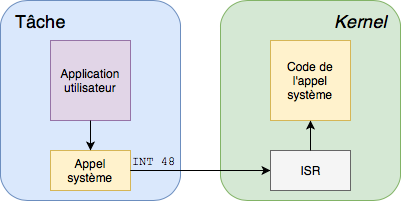
\includegraphics[scale=.7]{images/syscall.png}
  \caption{Fonctionnement des appels systèmes}
  \label{syscall}
\end{figure}

Avec la pagination active, il est important de copier les tables des pages et les
pages du \textit{kernel} dans le répertoire de pages de la tâche. C'est pour cette
raison que nous avons déplacé le \textit{kernel} dans le dernier gigaoctet de
\acrshort{ram} (chapitre \ref{activate_paging}). De cette façon, les trois premiers
gigaoctets de \acrshort{ram} peuvent être utilisés par une application utilisateur
et le reste par le \textit{kernel}.

%%%%%%%%%%%%%%%%%%%%%%%%%%%%%%%%%%%%%%%%%%%%%%%%%%%%%%%%%%%%%%%%%%
%%%%%%%%%%%%%%%%%%%%%%%%%%%%%%%%%%%%%%%%%%%%%%%%%%%%%%%%%%%%%%%%%%

\subsection{Allocation dynamique en mode utilisateur}
\label{alloc_user}
Le concept d'allocation dynamique a été expliqué dans le chapitre \ref{alloc_kernel}.
Les fonction décrites dans ce chapitre permettent seulement d'allour de la mémoire
en mode \textit{kernel}. Les tâches utilisateur pourraient très bien se passer
d'allocation dynamique et utiliser des structures statiques à la place. C'est
d'ailleurs de cette manière qu'avaient été implémentées les tâches dans une version
précédente de l'\acrshort{os}. Le problème qu'il y a avec l'utilisation de structures
statiques est que la même quantité de mémoire va être utilisée pour une application
faisant 200 octets et une application faisant 200'000 octets. De plus, toute la
mémoire dédiée aux tâches doit alors être réservée dès la compilation du \textit{kernel}
ce qui augmente très rapidement sa taille. Un autre avantage à allouer la mémoire
dynamiquement en \textit{ring} 3 est que des fonctions d'allocation dynamique 
peuvent alors être implémentées au niveau utilisateur (comme \mintinline{c}{malloc}
et \mintinline{c}{free}). \\

Dans le chapitre \ref{alloc_kernel}, nous avons vu les structures et mécanismes
mis en place pour allouer de la mémoire dynamiquement en mode \textit{kernel}.
Des fonctions supplémentaires ont été implémentées pour gérer la mémoire dynamique en
mode \textit{user}. Ces fonctions sont \mintinline{rust}{umalloc} et
\mintinline{rust}{ufree}. La fonction \mintinline{rust}{umalloc} alloue d'abord
de la mémoire en \textit{ring} 0 puis \textit{map} ces blocs mémoire
dans le répertoire de pages de la tâche utilisateur en commençant à l'adresse 0x0.
Le code du programme utilisateur est donc situé physiquement dans le \textit{heap}
du \textit{kernel} mais est placé virtuellement au début de l'espace d'adressage
de la tâche. Ce mécanisme est bien expliqué par la figure \ref{mem_view_user}.
Dans cet exemple, on peut voir que le code du programme utilisateur se situe
dans le tas du \textit{kernel} mais qu'il est \textit{mappé} à l'adresse 0x0
dans l'espace d'adressage de la tâche. A noter que le \textit{kernel} et son tas
sont encore présents dans la mémoire en mode \textit{user} pour rendre possibles
les appels systèmes (comme expliqué dans la partie précédente).

\begin{figure}[!h]
  \centering
  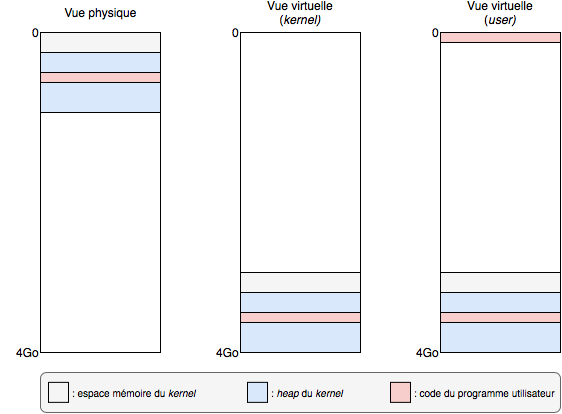
\includegraphics[scale=.7]{images/alloc_user.png}
  \caption{Vues de la mémoire après allocation d'un code utilisateur}
  \label{mem_view_user}
\end{figure}

%%%%%%%%%%%%%%%%%%%%%%%%%%%%%%%%%%%%%%%%%%%%%%%%%%%%%%%%%%%%%%%%%%
%%%%%%%%%%%%%%%%%%%%%%%%%%%%%%%%%%%%%%%%%%%%%%%%%%%%%%%%%%%%%%%%%%

\subsection{Librairie système et applications}
\subsubsection{Compilation d'une application utilisateur}
Le \textit{kernel} pouvant charger et exécuter des programmes, les appels systèmes
étant mis en place et l'allocation dynamique fonctionnelle en mode \textit{user},
des programmes utilisateurs peuvent maintenant être écrits. Ces applications
sont compilées séparément du \textit{kernel} avec un \textit{linker} qui leur
est propre. D'ailleurs, une application peut être codée dans le langage voulu
tant que le \textit{linker} fourni est utilisé. Un programme utilisateur est
compilé en format binaire. Sous ce format, le code du programme commence directement
à l'adresse 0x0. Il n'y a pas d'entête comme avec le format \acrshort{elf}.
Ci-dessous, les lignes importantes du \textit{linker} pour compiler en format
binaire. Ce \textit{linker} appelle une fonction assembleur très simple qui
appelle la fonction \mintinline{rust}{main} du programme \cite{ref42}. \\

\begin{code}
\begin{minted}[fontsize=\footnotesize,tabsize=4,frame=single,linenos]{text}
OUTPUT_FORMAT("binary")
SECTIONS {
    . = 0x0;
    ...
}
\end{minted}
\caption{\textit{Linker} pour un exécutable en format binaire}
\label{lst:tasks:app:linker}
\end{code} \bigbreak

Le langage rust a été utilisé pour développer une librairie système et quelques
applications. La compilation de rust est légèrement différente que pour le
\textit{kernel} car d'une part nous sommes dans un format binaire, et ensuite
il faut se défaire de tous les mécanismes de protection de rust qui prennent
une place considérable dans l'exécutable. Pour compiler un programme rust
en fichier objet destiné à un format binaire, le \textit{flag}
\mintinline{text}{-C relocation-model=static} doit être passé au compilateur.
Par défaut, le compilateur cherche la \mintinline{text}{GLOBAL_OFFSET_TABLE}
qui n'existe pas lorsque le format de l'exécutable est un format binaire.
Ce \textit{flag} va dire au compilateur d'ignorer ce mécanisme \cite{ref25}.
De cette façon, un programme utilisateur peut être compilé mais sa taille sera
excessivement grande (dans l'ordre des 100'000 octets). Ceci est du à plusieurs
raisons. Tout d'abord, rust est compilé par défaut sans aucune option d'optimisation.
Le \textit{flag} \mintinline{text}{-C opt-level=3} fixe un niveau d'optimisation
de 3 (plus haut niveau d'optimisation). Un peu plus d'optimisation peut être
fait en disant à xargo de compiler en mode \textit{release} et non \textit{debug}
avec l'option \mintinline{text}{--release}. Le niveau d'optimisation a un impact
sur le code écrit mais ce sont les librairies qui prennent le plus de place dans
un exécutable. Pour rappel, nous compilons sans librairie standard mais la librairie
\mintinline{text}{core} est tout de même utilisée. Quand on compile un code rust,
l'intégralité de cette librairie est compilée aussi, même si certaines parties
sont inutiles. Pour résoudre ce problème il faut cette fois-ci modifier le fichier
\mintinline{text}{cargo.toml} et lui rajouter les lignes suivantes \cite{ref26}.

\begin{code}
\begin{minted}[fontsize=\footnotesize,tabsize=4,frame=single,linenos]{text}
[profile.release]
lto = true
panic = 'abort'
\end{minted}
\caption{Options ajoutées au fichier \mintinline{text}{cargo.toml}}
\label{lst:tasks:app:cargotoml}
\end{code} \bigbreak

A noter que les \textit{flags} passés au compilateur de rust (avec l'option
\mintinline{text}{-C}), sont appliqués au compilateur rustc et non à xargo. Pour
dire à xargo (ou cargo) de rajouter des options lors de la compilation, il faut
mettre ces options dans la variable d'environnement \mintinline{text}{RUSTFLAGS}.
Comme pour le \textit{kernel}, \acrshort{gcc} est utilisé pour \textit{linker}
les fichier objets en un exécutable.

\subsubsection{Librairie système}
Pour faciliter le développement d'applications pour l'\acrshort{os}, une librairie
système a été développée. Cetter dernière agit comme une mini librairie C offrant
les fonctionnalités de base à un programme utilisateur. Cette librairie offre
un niveau d'abstraction plus élevé cachant l'utilisation d'appels systèmes
à l'utilisateur. Ainsi, aucune application n'a besoin de faire appel des appels
systèmes. C'est la librairie système qui s'en charge. La librairie dévelopée
offre les fonctionnalités suivantes.

\begin{center}
	\scalebox{1}{
		\begin{tabular}{| l | l |}
			\hline
			Fonction & Description \\ \hline
			\mintinline{rust}{print}/\mintinline{rust}{println} & Macros permettant
            d'afficher une chaîne de caractères formatée \\ \hline
			\mintinline{rust}{clear} & Efface l'écran \\ \hline
			\mintinline{rust}{puts} & Affiche une chaîne de caractères \\ \hline
			\mintinline{rust}{putc} & Affiche un caractère \\ \hline
			\mintinline{rust}{exec} & Exécute un programme utilisateur contenu
            dans le disque dur \\ \hline
            \mintinline{rust}{keypressed} & Indique si une touche tu clavier a
            été appuyée \\ \hline
            \mintinline{rust}{getc} & Fonction bloquante. Retourne la touche
            appuyée par l'utilisateur \\ \hline
            \mintinline{rust}{file_stat} & Retourne les métadonnées d'un fichier \\ \hline
            \mintinline{rust}{file_open} & Ouvre un fichier donné en paramètre
            et retourne son descripteur \\ \hline
            \mintinline{rust}{file_close} & Ferme un fichier à partir de son
            descripteur \\ \hline
            \mintinline{rust}{file_read} & Lit les octets d'un fichier depuis son
            descripteur \\ \hline
            \mintinline{rust}{file_seek} & Avance le curseur d'un fichier depuis
            son descripteur \\ \hline
            \mintinline{rust}{file_iterator} & Retourne un itérateur des fichiers
            du disque dur \\ \hline
            \mintinline{rust}{file_next} & Itère sur le prochain fichier du disque \\ \hline
            \mintinline{rust}{get_ticks} & Retourne l'état actuel du \textit{timer} \\ \hline
            \mintinline{rust}{sleep} & Arrête l'exécution pendant un temps donné \\ \hline
            \mintinline{rust}{set_cursor} & Fixe la position du curseur sur l'écran \\ \hline
            \mintinline{rust}{get_cursor} & Retourne la position du curseur sur
            l'écran \\ \hline
            \mintinline{rust}{cursor_disable} & Active ou désactive le curseur \\ \hline
            \mintinline{rust}{copy_scr} & Copie un \textit{frame buffer} sur
            l'écran \\ \hline
            \mintinline{rust}{malloc} & Alloue de la mémoire \\ \hline
            \mintinline{rust}{free} & Libère de la mémoire \\ \hline
		\end{tabular}
	}
    \captionof{table}{Fonctions proposées par la librairie système}
    \label{tab:tasks:ulibc}
\end{center}

La fonction \mintinline{rust}{malloc} utilise un appel système allouant une nouvelle
page dans le répertoire de pages de la tâche. Cet appel système appelle lui même
la fonction \mintinline{rust}{umalloc} décrite dans la partie \ref{alloc_user}.
la fonction \mintinline{rust}{malloc} gère la mémoire de la même manière que le
\textit{kernel}. Un tas est utilisé au niveau utilisateur. Quand un utilisateur
alloue de la mémoire, \mintinline{rust}{malloc} va regarder s'il y a assez de
place dans la dernière page allouée. Si c'est le cas, aucun appel système n'est
appelé, une partie de la dernière page va être reservée. Dans le cas contraire,
l'appel système pour allouer une page est appelé autant de fois que nécessaire.
Cette gestion utilise des entêtes qui fonctionnent exactement comme ceux du
\textit{heap} du \textit{kernel} décrits en \ref{alloc_kernel}. La seule différence
est que l'espace alloué n'est pas aligné sur 4096 octets (la taille d'une page)
car l'utilisateur aura tendance à allouer des espace plus petits et cela produirait
une trop grande perte de mémoire. De plus, si l'espace alloué était alligné sur
la taille d'une page, un appel système aurait lieu à chaque allocation ce qui n'est
pas souhaitable.

\subsubsection{Applications développées}
\paragraph{Shell} \mbox{} \\
Actuellement, les applications utilisateurs ne peuvent être appélées que depuis
le \textit{kernel}. Ceci n'est pas très pratique d'un point de vue utilisateur.
Afin d'avoir un système d'exploitation un peu plus intéractif, un shell très
simple a été développé. Ce shell permet de lire les fichiers du disque dur et
d'exécuter d'autres applications utilisateur. Le shell implémenté propose
les fonctionallités suivantes.

\begin{itemize}[label=\textbullet]
	\item \mintinline{text}{ls}         : liste les fichiers du disque dur
	\item \mintinline{text}{cat <file>} : affiche le contenu d'un fichier
	\item \mintinline{text}{clear}      : efface l'écran
	\item \mintinline{text}{<prog>}     : exécute un programme
    \item \mintinline{text}{sleep <ms>} : attend pendant un temps donné 
    \item \mintinline{text}{exit}       : sort du shell
    \item \mintinline{text}{help}       : affiche la liste des commandes disponibles
\end{itemize}

\begin{figure}[!h]
  \centering
  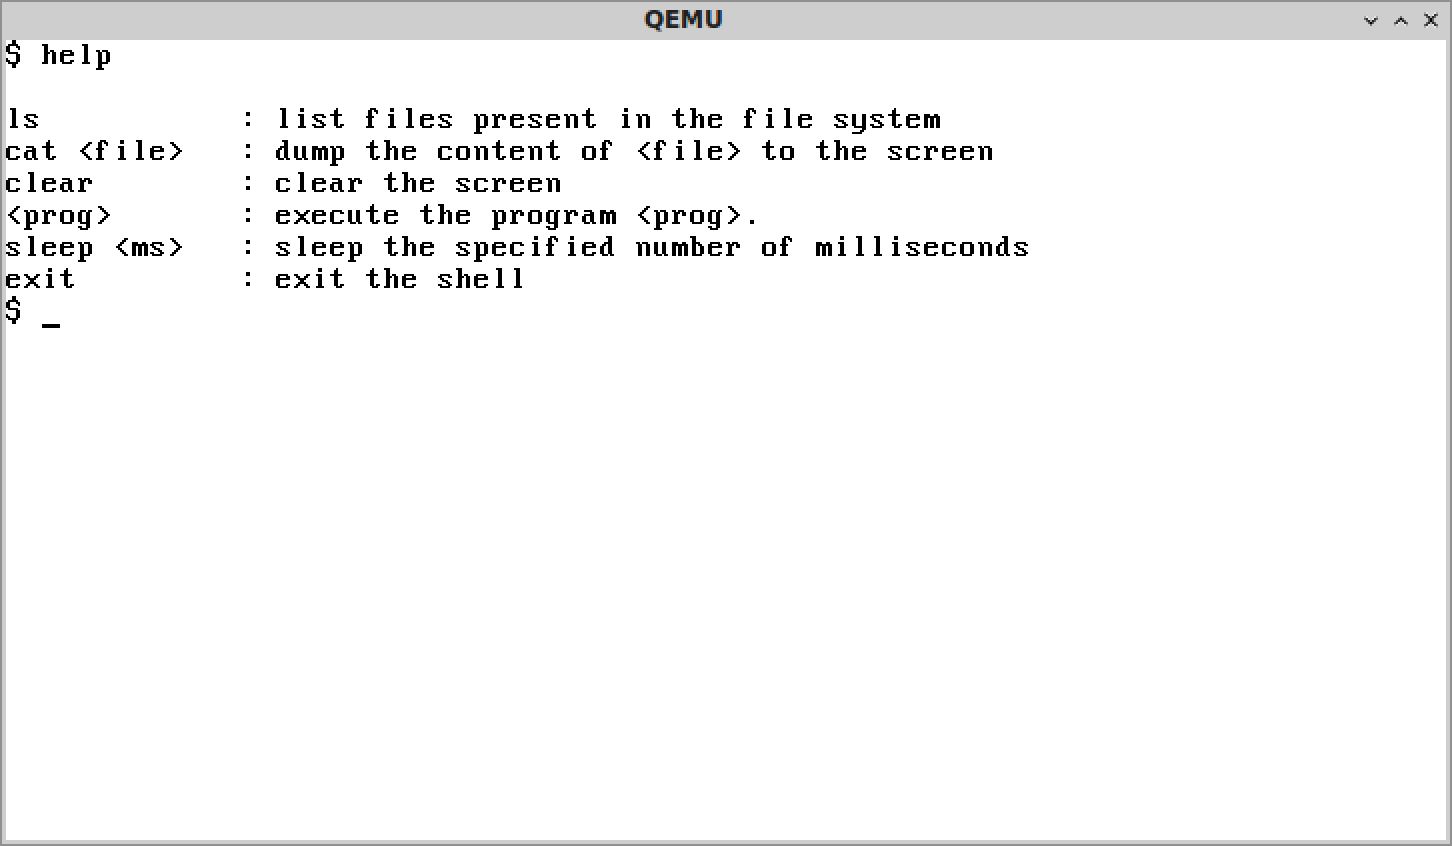
\includegraphics[scale=.6]{images/shell.png}
  \caption{Shell développé}
  \label{mem_view_user}
\end{figure}

\paragraph{Démo} \mbox{} \\
En plus du shell, une démo a été développée afin de valider toutes les fonctionnalités
de l'\acrshort{os}. Cette démo appelle toute les fonctions de la librairie système
et teste l'allocation mémoire dynamique.